\section{Results}
\label{sect:results}

% Order follows the agreed story (findings.md, "Paper story").

\subsection{Effect of the PET-Preservation and Rigidity Losses}
\label{sect:res_q1}
\todo{Q1 text from Table~\ref{tab:ablations}: PET lowers $|\Delta\mathrm{MTV}|$ / $|\Delta\mathrm{TLG}|$ significantly as network output and with IO, at about 2--3 Dice points; rigidity lowers $|\Delta\mathrm{MTV}|$ at $\leq0.5$ Dice points; HD95 follows Dice; NDV below the threshold for every run. Early stopping (one sentence): best-tumour checkpoint costs 3.0 Dice points, $|\Delta\mathrm{MTV}|$ $-0.4$ (n.s.).}
\begin{table}[t]
\centering
\caption{Effect of the PET and rigidity losses on the test set (CT Dice: 28 patients, 38 pairs; PET: 26 patients, 30 pairs). Each network is trained with the given losses and evaluated as is (left) and with instance optimisation (IO) using the same losses (right). Mean$\pm$SD over patients. $^{\dagger}$/$^{\ddagger}$: significantly better/worse than ``Neither'' in the same block (two-sided Wilcoxon signed-rank test on patient values, Holm-corrected over three comparisons within each column, $p<0.05$).}
\label{tab:ablations}
\scriptsize
\setlength{\tabcolsep}{3pt}
\begin{tabular}{lcccccc}
\toprule
 & \multicolumn{3}{c}{Network} & \multicolumn{3}{c}{Network + IO} \\
\cmidrule(lr){2-4} \cmidrule(lr){5-7}
Losses & Dice (\%) $\uparrow$ & $|\Delta\mathrm{MTV}|$ (\%) $\downarrow$ & $|\Delta\mathrm{TLG}|$ (\%) $\downarrow$ & Dice (\%) $\uparrow$ & $|\Delta\mathrm{MTV}|$ (\%) $\downarrow$ & $|\Delta\mathrm{TLG}|$ (\%) $\downarrow$ \\
\midrule
Neither & 74.8$\pm$4.5 & 10.6$\pm$10.2 & 10.8$\pm$11.7 & 79.2$\pm$4.3 & 10.2$\pm$10.1 & 11.9$\pm$12.5 \\
PET & 72.9$\pm$4.4$^{\ddagger}$ & 7.6$\pm$9.0$^{\dagger}$ & 7.6$\pm$9.3$^{\dagger}$ & 76.4$\pm$4.7$^{\ddagger}$ & 6.3$\pm$9.1$^{\dagger}$ & 7.2$\pm$9.4$^{\dagger}$ \\
Rigidity & 74.8$\pm$4.5 & 9.4$\pm$9.5$^{\dagger}$ & 9.5$\pm$10.9$^{\dagger}$ & 78.7$\pm$4.2$^{\ddagger}$ & 7.9$\pm$9.0$^{\dagger}$ & 10.1$\pm$11.0 \\
PET + rigidity & 72.8$\pm$4.3$^{\ddagger}$ & 7.4$\pm$9.0$^{\dagger}$ & 7.7$\pm$10.1$^{\dagger}$ & 75.6$\pm$4.8$^{\ddagger}$ & 6.2$\pm$8.7$^{\dagger}$ & 7.9$\pm$9.0 \\
\bottomrule
\end{tabular}
\end{table}


\subsection{Losses in Training or Only in IO}
\label{sect:res_q2}
\todo{Q2 text from Fig.~\ref{fig:q2} and q2\_effects.txt: losses only in IO vs.\ in training and IO: Dice +1.2 (PET) and +1.7 (both) points, significant; $|\Delta\mathrm{MTV}|$ +0.5 to +1.3 points, not significant. Without IO, the training losses are the only way to obtain preservation.}
\begin{figure}[t]
\centering
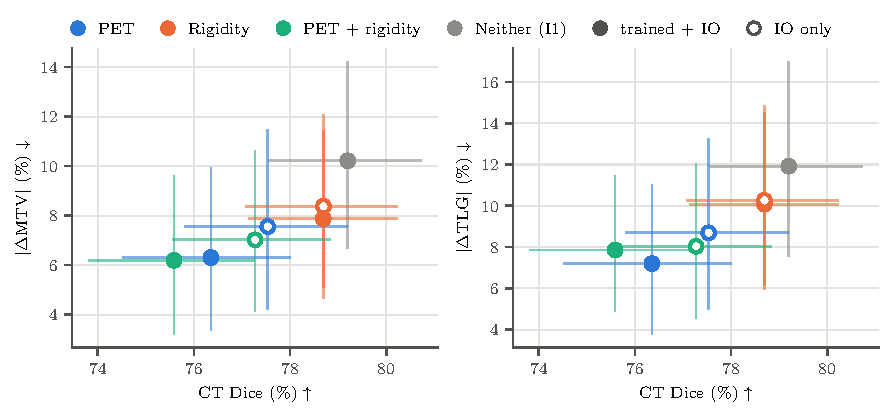
\includegraphics[width=\textwidth]{figures/q2.pdf}
\caption{Losses in training and IO versus only in IO (test set; CT Dice: 28 patients, PET: 26 patients). For each loss set, filled: network trained with the losses, then IO with them; hollow: network trained without them (T1), same IO. Grey: neither loss (I1). Points: patient means with 95\,\% patient-bootstrap confidence intervals for each method; confidence intervals for paired differences are reported in the text.}
\label{fig:q2}
\end{figure}


\subsection{Per-Lesion Volume Change}
\label{sect:res_lesions}
\todo{Text from findings.md, ``Per-lesion volume change: draft results text''.}
\begin{figure}[t]
\centering
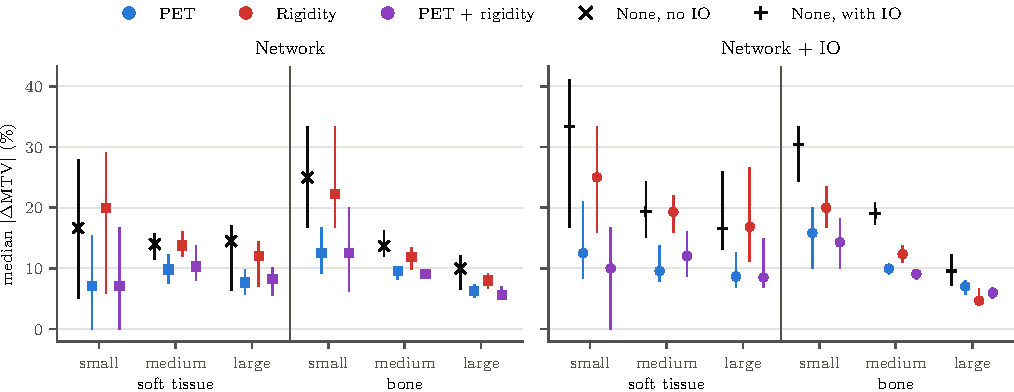
\includegraphics[width=\textwidth]{figures/lesions.pdf}
\caption{Per-lesion absolute volume change on the test set (1327 lesions from 26 patients and 30 pairs after excluding 108 components smaller than five voxels), stratified by location (soft tissue or bone-associated, with $\geq$50\,\% of the lesion on bone) and size (small $<0.5$~ml, medium $0.5$ to $<5$~ml, large $\geq5$~ml).
 Points show the median $|\Delta\mathrm{MTV}|$ per lesion; left: network output, right: instance optimization (IO) with the same losses.
 Within each size stratum, the loss groups are ordered PET, rigidity, and PET plus rigidity; squares and circles denote without and with IO, while $\times$ and $+$ denote the corresponding configurations without losses.
 Error bars: 95\,\% confidence intervals from a patient-cluster bootstrap.}
\label{fig:lesions}
\end{figure}


\subsection{Contribution of Each PET Term}
\label{sect:res_loo}
\todo{Leave-one-out table (tables/loo.tex) once L1--L4 have run.}

\subsection{Comparison with Baselines}
\label{sect:res_baselines}
\todo{Text from Table~\ref{tab:baselines}, Fig.~\ref{fig:baselines_distribution}, Fig.~\ref{fig:qualitative}: every variant of ours significantly more accurate than NiftyReg, ConvexAdam, and the affine; no folding; ranks; affine + IO reaches 52.7\,\% Dice, so the network is essential; runtimes.}
\begin{table}[t]
\centering
\caption{Comparison with baselines on the test set (28 patients, 38 follow-up$\rightarrow$baseline pairs; PET: 26 patients, 30 pairs).
 Values are mean$\pm$SD over patients (a patient's eligible pairs are averaged first).
 HD95: 95th-percentile Hausdorff distance; MTV: metabolic tumor volume; TLG: total lesion glycolysis; NDV: non-diffeomorphic volume.
 Rank: descriptive challenge significance ranking, with the 95\,\% interval of the rank over 1000 patient bootstrap samples in brackets, over all methods except Initial, which is a reference (its MTV/TLG change is 0 by construction because nothing is resampled).
 Training / IO: PET and rigidity losses (PET + rig.) used in training and in instance optimization (IO); IO ``--'': no IO, ``basic'': IO with the similarity and regularization terms only.
 $^{\dagger}$/$^{\ddagger}$: Ours + IO with PET + rig. only in IO (our method, chosen on the validation set) is significantly better/worse than this method (two-sided Wilcoxon signed-rank test on patient values, Holm-corrected over nine comparisons for CT/HD95/NDV and eight for PET within each column, $p<0.05$; NDV tested after the 0.005\,\% equivalence threshold).
 NDV is summarized as mean$\pm$SD over patients; $>$ thr. is the percentage of individual pairs with \%NDV above 0.005\,\%.
 Runtime per pair on one NVIDIA RTX A6000 (measured in the runs with the earlier scorer, same IO settings), including the affine step.
 Affine + IO: our instance optimization directly after the affine pre-registration, without the network.
 Bold: best mean among ranked methods.}
\label{tab:baselines}
\scriptsize
\setlength{\tabcolsep}{2.5pt}
\resizebox{\textwidth}{!}{%
\begin{tabular}{lllcccccccc}
\toprule
Method & Training & IO & Rank $\downarrow$ & Dice (\%) $\uparrow$ & HD95 (mm) $\downarrow$ & $|\Delta\mathrm{MTV}|$ (\%) $\downarrow$ & $|\Delta\mathrm{TLG}|$ (\%) $\downarrow$ & NDV (ppm) $\downarrow$ & $>$ thr. (\%) & Runtime (s) \\
\midrule
Initial & -- & -- & -- & 9.5$\pm$8.1$^{\dagger}$ & 44.37$\pm$21.32$^{\dagger}$ & 0.0$\pm$0.0 & 0.0$\pm$0.0 & 0$\pm$0 & 0 & -- \\
Affine & -- & -- & 8 [4--9] & 46.4$\pm$11.0$^{\dagger}$ & 14.00$\pm$4.83$^{\dagger}$ & \textbf{4.5}$\pm$4.6 & \textbf{4.4}$\pm$4.6$^{\ddagger}$ & \textbf{0}$\pm$0 & 0 & 10.4$\pm$0.3 \\
NiftyReg & -- & -- & 6 [1--8] & 70.1$\pm$5.0$^{\dagger}$ & 8.85$\pm$3.73$^{\dagger}$ & 8.7$\pm$12.8 & 10.2$\pm$16.9 & 328$\pm$885 & 21 & 107.7$\pm$24.9 \\
ConvexAdam & -- & -- & 7 [7--9] & 61.7$\pm$4.5$^{\dagger}$ & 9.16$\pm$3.14$^{\dagger}$ & 9.3$\pm$12.0 & 10.8$\pm$16.5 & \textbf{0}$\pm$0 & 0 & 11.3$\pm$0.6 \\
Affine + IO & -- & PET + rig. & 8 [4--9] & 56.6$\pm$12.1$^{\dagger}$ & 12.88$\pm$4.81$^{\dagger}$ & 5.3$\pm$4.1 & 6.8$\pm$4.0 & 0.45$\pm$0.31 & 0 & 155.5$\pm$2.6 \\
\midrule
Ours & -- & -- & 4 [3--6] & 75.5$\pm$4.7$^{\dagger}$ & 7.20$\pm$2.30$^{\dagger}$ & 10.3$\pm$9.5 & 12.5$\pm$11.1 & 0.056$\pm$0.057 & 0 & 11.0$\pm$0.4 \\
Ours & PET + rig. & -- & 5 [1--6] & 73.6$\pm$4.6$^{\dagger}$ & 7.44$\pm$2.37$^{\dagger}$ & 8.0$\pm$9.0 & 9.8$\pm$10.9 & 0.64$\pm$0.62 & 0 & 11.3$\pm$0.3 \\
Ours + IO & -- & basic & 1 [1--4] & \textbf{80.2}$\pm$4.2$^{\ddagger}$ & \textbf{6.64}$\pm$2.28$^{\ddagger}$ & 11.3$\pm$11.9 & 14.5$\pm$14.1 & 0.65$\pm$0.13 & 0 & 153.9$\pm$2.6 \\
Ours + IO & PET + rig. & PET + rig. & 3 [1--5] & 77.3$\pm$4.9$^{\dagger}$ & 7.07$\pm$2.38$^{\dagger}$ & 7.9$\pm$9.7 & 10.3$\pm$10.4 & 10.4$\pm$49.3 & 3 & 156.6$\pm$2.7 \\
Ours + IO & -- & PET + rig. & 2 [1--4] & 78.3$\pm$4.4 & 6.89$\pm$2.31 & 8.7$\pm$10.7 & 11.3$\pm$11.2 & 4.15$\pm$9.45 & 5 & 157.2$\pm$2.6 \\
\bottomrule
\end{tabular}}
\end{table}

\begin{figure}[t]
\centering
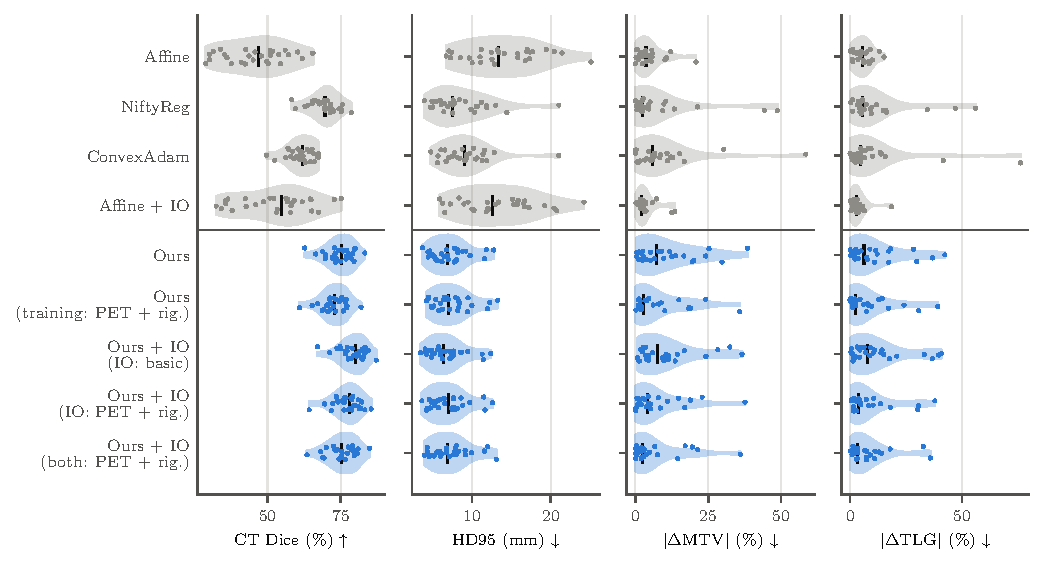
\includegraphics[width=\textwidth]{figures/baselines_distribution.pdf}
\caption{Patient-level results on the test set (CT Dice and HD95: 28 patients; PET: 26 patients; a patient's eligible pairs are averaged).
 Violins: kernel density over patients, line: median; each dot is one patient. In brackets: where the PET and rigidity losses (PET + rig.) act; basic: IO with the similarity and regularization terms only; both: training and IO.
 Initial alignment is omitted (CT Dice 9.5\,\%, HD95 44.4\,mm; MTV/TLG change 0 by construction, Table~\ref{tab:baselines}).}
\label{fig:baselines_distribution}
\end{figure}

\begin{figure}[p]
\centering
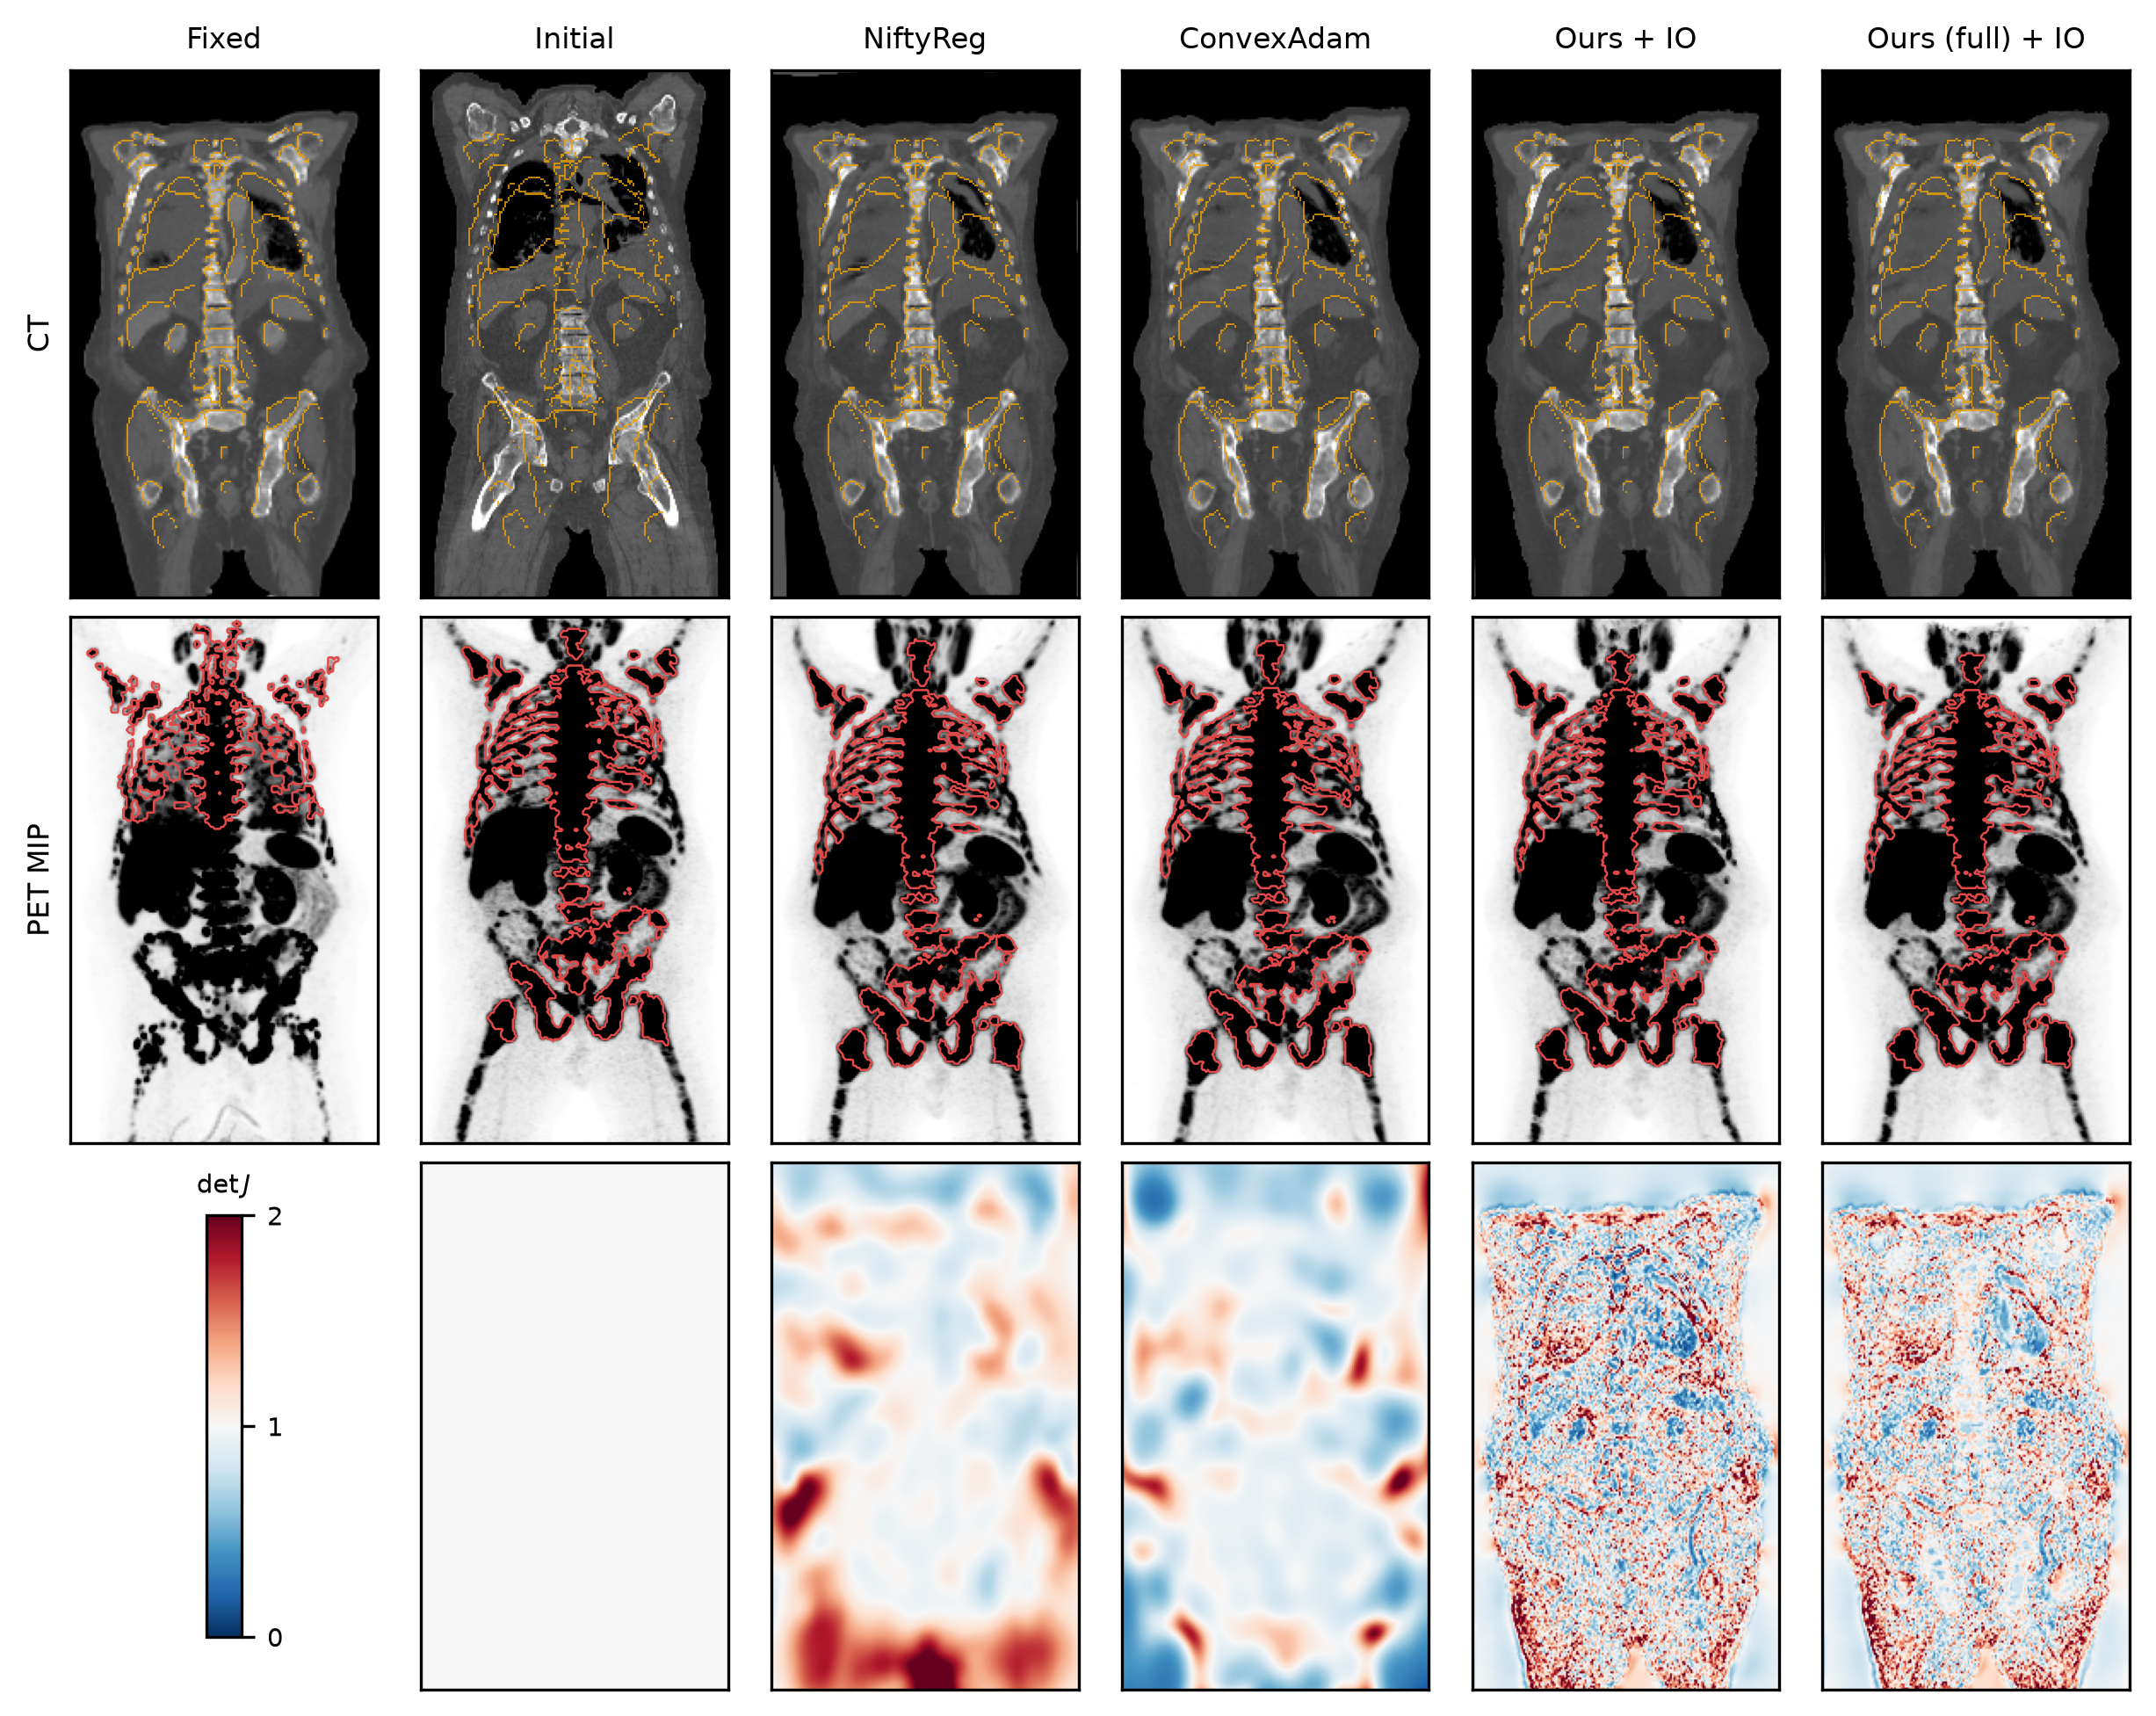
\includegraphics[width=\textwidth]{figures/qualitative.png}
\caption{Anatomical alignment example from the test set, registered by our method (PET-preservation and rigidity losses only in instance optimization [IO]); one coronal slice.
 Patient 0146 was selected for its large between-image change in lesion volume (2400 voxels at baseline and 24\,191 at follow-up).
 The example illustrates anatomical alignment and deformation.
 (a)~Fixed and (b)~moving CT images overlaid with the corresponding PET images (SUV 0--8, 35\,\% opacity) and provided lesion contours (red).
 (c,~d)~Fixed CT image (green) overlaid with the moving CT image (magenta) before~(c) and after~(d) registration; gray where they agree.
 (e,~f)~Organ labels that differ before~(e) and after~(f) registration: green where the fixed image has a label that the moving image lacks there, magenta where only the moving image is labeled; bright, medium, and dark shades for bones, organs, and muscles.
 (g)~Jacobian determinant of the fixed-to-moving transformation: white is volume-preserving (1), blue is below 1 and red is above 1; changes in the displayed warped anatomy have the opposite direction.
 (h)~Warped moving CT image overlaid with the corresponding PET image and warped lesion contours.}
\label{fig:qualitative}
\end{figure}


\subsection{Rigidity Penalties}
\label{sect:res_rigidity}
\todo{After the validation sweeps and test runs: curve of Dice vs.\ distance distortion (validation), test table with bone/soft-tissue alignment, distance distortion, NDV in bone and boundary band, stencil leakage, erosion retention. Leakage on all 560 scans: 21.2\,\% of stencil reads leave the bone; erosion keeps 35.5\,\% of bone voxels and removes 23\,\% of bones (ribs: 2.4\,\% kept, 58\,\% removed).}

\subsection{Accuracy--Preservation Trade-off}
\label{sect:res_tradeoff}
\todo{Trade-off curve (PET weight $\times\{0,0.01,0.03,0.1,0.3,1\}$) once the runs are done; mark the tuned operating point.}
